	El núcleo del Kit de Desarrollo FX2LP EZ-USB es un CY7C68013A. Dicho circuito integrado, cuya arquitectura se presenta en la Figura \ref{arqEzUSB}. Los chips de la familia FX2LP integran un transceptor USB, un SIE {\it Serial Interfaz Engine}, buffers de datos, un microcontrolador 8051 mejorado y una interfaz programable hacia los periféricos. Además posee un un PLL y un divisor configurable a través de los cuales provee al sistema de las señales de reloj adecuadas para el correcto funcionamiento del sistema.\\
	
	\begin{figure}[h]
		\centering
		%TODO meter la imagen
%		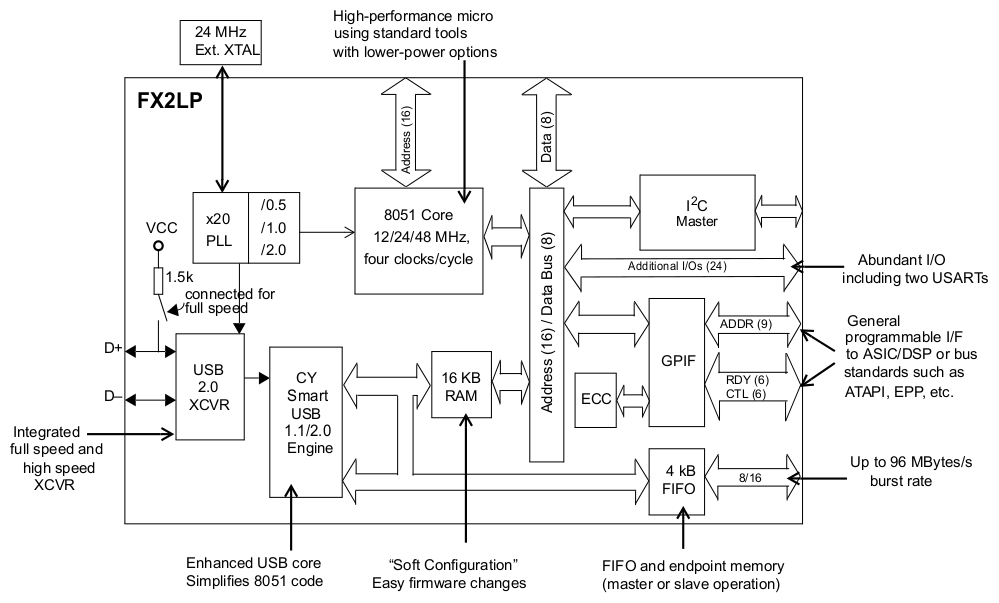
\includegraphics[width=.7\textwidth]{arqfx2lp.png}
		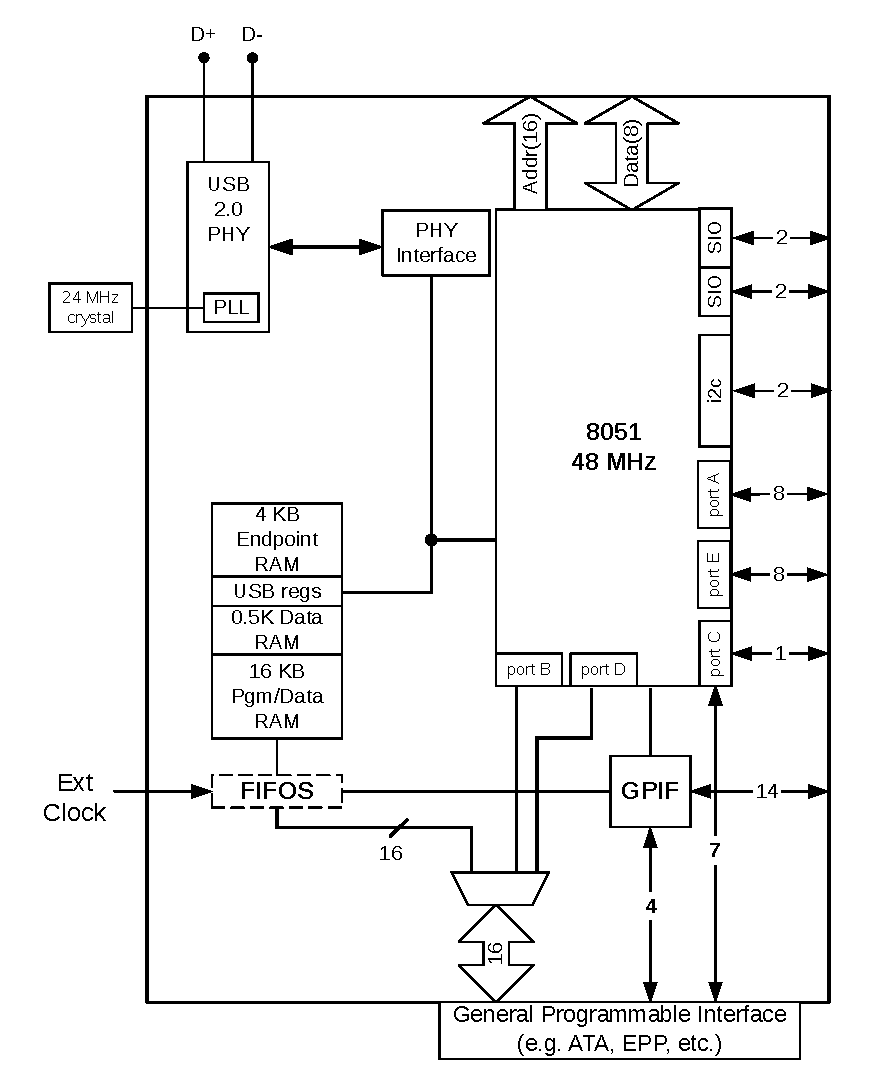
\includegraphics[width=.55\textwidth]{arq.eps}
		%TODO Meter la referencia
		\caption{Arquitectura FX2LP} 
		\label{arqEzUSB}
	\end{figure}

	Esta arquitectura permite al usuario trasmitir datos desde y hacia la PC desde el mimso puerto USB, o bien via RS-232, desde la PC. A la hora de comunicarse con sistemas periféricos se puede aprovecar el puerto I2C, la interfaz de propósito general o una interfaz esclavo que puede ser conectada a un sistema maestro. Esto brinda muchas alternativas, desde la conexión a puertos estandar, como ser ATA, PCMCIA o EPP, o también la conexión de dispositivos tales como DSP's y FPGA's.\\
	
	La comunicación USB es llevada a cabo a través del transceptor, unido al SIE. Como se observa en la Figura \ref{usbxcvr}. El usuario, a fin de intercambiar datos, solo debe colocar o extraer los datos de registros destinados a tal fin y modificar las banderas de handshaking, que en la figura se observan como ACK (abreviación del ingles {\it acknowledge}, que significa reconocer, aceptar o agradecer), que indican si el sistema está disponible, si los datos fueron colocados o leídos, dependiendo el caso tratado. El SIE y el transceptor USB se encargan de empaquetar, enviar, recibir y desempaquetar toda la información, así como leer los tokens que emite el host, calcular y corroborar los códigos cíclicos de detección de errores y todo lo relacionado al protocolo en sí.\\
	
	\begin{figure}[h]
		\centering
		\includegraphics[width=.65\textwidth]{usbxcvr}
		\caption{Implementación del enlace USB realizado por el EZ-USB}
		\label{usbxcvr}
	\end{figure}
	
	El esquema de bus permite utilizar el microcontrolador 8051 para procesar datos, hacer control de errores, empaquetar datos de una forma particular, generar datos nuevos, entre otras, o bien, simplemente enviar datos desde un periférico de forma directa al SIE y luego transmitirlos a la PC por la tubería USB.\\
	
	Para este trabajo final, se configuró el funcionamiento del EZ-USB en modo esclavo, conectando al maestro, la FPGA, a la memoria FIFO destinada para tal fin. Por lo que se describirá en detalle a continuación.\\
	
	Al poseer el sistema un SIE, que es un serializador de datos, la memoria FIFO de 4kB es usada por el sistema como buffer. Se conecta de forma directa a los periféricos y es configurable, lo que permite al usuario disponer del espacio conforme requiera las necesidades de ancho de banda de los sistemas diseñados, evitando así las congestiones en casos de mucho flujo de datos. En el otro extremo, puede ser conectada al tubo USB o al microntolador, dirigiendo los datos directamente a la PC o realizando algúna acción sobre ellos antes de enviarlos, respectivamente.\\
	
	El sistema FX2LP permite configurar los buffers conforme la se ve en la Figura \ref{epconfigs}. Es de destacar que en cualquiera de las configuraciones posibles, se tiene al menos dos buffers. Los diseñadores del integrado pensaron esto como una solución a la congestión. Para ello, los buffers se pueden configurar duplicados, triplicados o cuadruplicados, dependiendo de las necesidades. Luego, el sistema de forma automática se encarga de permutar los buffers de forma tal que no queden datos retenidos en el dispositivo maestro. Cómo se detallará más adelante, para este trabajo se configuraron dos enpoints como el modo 11 de la fFigura \ref{epconfigs}, es decir, un extremo con 3 buffers de 1024 bytes y otro con 2 buffers de 512 bytes.\\
	
	Los buffers pueden ser conectados directa hacia el SIE, de forma que realice la comunicación entre la PC y los periféricos de forma automática, incluso programando un umbral de cantidad de datos que cunado sea revasado envíe los datos hacia la PC; o bien se puede acceder a ellos desde el microcontrolador, de forma de poder realizar alguna acción específica sobre los datos antes de mandarlos hacia la PC o los periféricos.\\
		
	\begin{figure}[h]
		\centering
		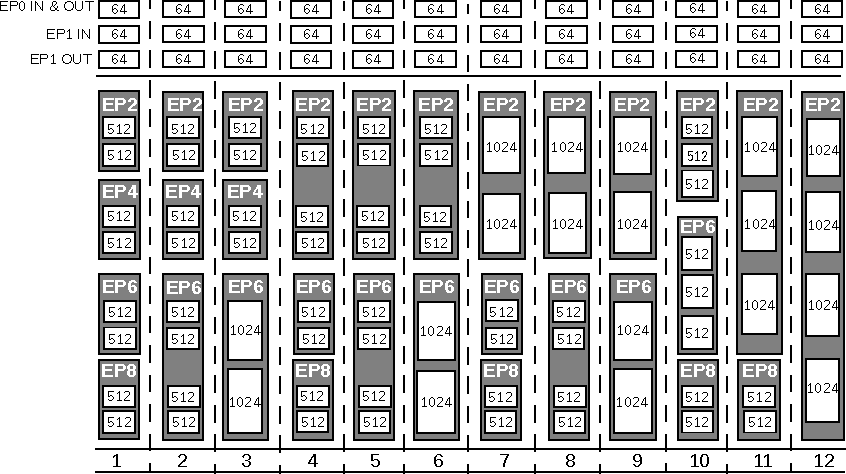
\includegraphics[width=0.6\textwidth]{bufconf}
		\caption{Configuraciones admitidas para los buffers de los diferentes periféricos}
		\label{epconfigs}
	\end{figure}